% This file was adapted from ICLR2022_conference.tex example provided for the ICLR conference
\documentclass{article} % For LaTeX2e
\usepackage{conference,times}
\usepackage{easyReview}
\usepackage{algorithm}
\usepackage{algorithmic}

% Optional math commands from https://github.com/goodfeli/dlbook_notation.
\input{math_commands.tex}

\usepackage{amsthm,amssymb}

\newtheorem{theorem}{Theorem}[section]
\newtheorem{corollary}{Corollary}[theorem]
\newtheorem{lemma}[theorem]{Lemma}
\newtheorem{definition}[theorem]{Definition}

% Please leave these options as they are
\usepackage{hyperref}
\hypersetup{
    colorlinks=true,
    linkcolor=red,
    filecolor=magenta,
    urlcolor=blue,
    citecolor=purple,
    pdftitle={Certified Hybrid Non-Convex Robust Dynamic Operating Envelopes for Unbalanced Distribution Networks},
    pdfpagemode=FullScreen,
    }



\title{Certified Hybrid Non-Convex Robust Dynamic Operating Envelopes for Unbalanced Distribution Networks}

\author{Anonymous Authors \\
Affiliation Withheld for Review \\
\texttt{anonymous@anonymous.edu}}

\begin{document}


\maketitle

\begin{abstract}
Robust dynamic operating envelopes (RDOEs) are increasingly used to allocate low-voltage flexibility while preserving voltage and thermal security under uncertain load and distributed energy resource behavior. Purely linear robust approximations scale well but can misestimate nonlinear boundary regions in unbalanced feeders, whereas full non-convex robust unbalanced three-phase optimal power flow (UTOPF) is often too expensive for high-cadence operation. We present a hybrid method that couples a certified linear screening stage with selective non-convex escalation and prove two properties: (i) accepted screened points are robust-feasible under explicit residual assumptions, and (ii) accepting all certifiable points is compute-optimal among admissible deterministic escalation rules. The method is evaluated on a reproducible four-experiment suite covering security-runtime tradeoffs, online uncertainty calibration, fairness-sensitive allocation, and cross-solver shadow-mode behavior. Across 600 configuration-seed samples per experiment family, nominal screening behavior remains consistent with the safety theorem, observed runtime reduction is substantial for boundary-aware operation, uncertainty calibration tracks target risk with bounded coverage error, and cross-solver discrepancy remains within predefined operational tolerances in synthetic stress regimes. The broader contribution is a deployable bridge between optimization guarantees and operational evidence: theorem-scoped safety and optimality are connected to experiment-level diagnostics, reproducibility artifacts, and policy-sensitive allocation analysis.
\end{abstract}

\section{Introduction}
Distribution system operators are being asked to operate low-voltage networks with substantially higher penetrations of rooftop photovoltaic generation, batteries, and controllable demand than the planning assumptions that shaped static connection policies. In this setting, fixed export caps and static rule curves are often either too conservative, leaving flexibility unused, or too permissive, admitting occasional voltage and thermal violations when uncertainty and phase imbalance align unfavorably. Dynamic operating envelopes were introduced to replace static limits with time-varying, asset-specific bounds that follow forecasted and measured network conditions \citep{KA15,KA35}. Robust dynamic operating envelopes extend this concept by explicitly internalizing uncertainty, but this gain in security typically increases computational burden because feasible-set evaluation now requires uncertainty-aware multiphase network checks \citep{KA01,KA03,KA04}.

The central technical tension is now clear in the literature. High-fidelity non-convex UTOPF pipelines better preserve nonlinear security boundaries but can be expensive for day-ahead plus intraday receding updates \citep{KA01,KA05,KA21}. Linearized robust envelopes reduce runtime but may under-approximate or over-approximate critical parts of the feasible region, especially around stressed operating points \citep{KA02,KA22}. Data-driven and stochastic variants can improve adaptability, yet they depend on forecast quality, calibration design, and drift handling \citep{KA04,KA06,KA07}. At the same time, operators increasingly require envelope allocation policies that are not only secure and fast, but also transparent in fairness and comparable to existing DSO operating procedures \citep{KA08,KA10,KA14}. As reviewed in \citet{KA35}, this creates a cross-domain requirement: optimization rigor, statistical calibration, and operations evidence must cohere in one pipeline.

This paper develops a hybrid robust envelope method that keeps non-convex verification in the loop while reducing unnecessary expensive solves. The method uses a certified screening predicate derived from linearized margins and explicit nonlinear residual bounds, then escalates only uncertified points to non-convex robust solves. The approach is intentionally theorem-linked and evidence-linked: we provide formal statements and complete proofs for safety and compute optimality of the escalation policy under clear assumptions, then evaluate those assumptions and consequences through reproducible experiments, including stress modes designed to invalidate assumptions and verify falsifiability.

The resulting framing also has implications outside classical power optimization. The same architecture---fast certifiable screening plus selective high-fidelity verification---appears in safety-critical machine learning, autonomous control, and operations research pipelines where model mismatch and compute budgets interact. In our context, this means RDOE design can be treated not as a single-solver choice, but as a compositional decision process with formal admissibility constraints and measurable deployment diagnostics.

Our contributions are:
\begin{itemize}
\item We formalize a robust feasible-set screening condition for non-convex RDOE computation and prove that certified points satisfy strict robust margins when residual assumptions hold, providing a precise safety guarantee rather than a heuristic trigger.
\item We formulate escalation as an admissible policy optimization problem and prove that accepting every certifiable point is compute-optimal among deterministic admissible policies under standard cost ordering.
\item We connect formal claims to a reproducible validation suite spanning security-runtime behavior, uncertainty calibration, fairness-sensitive allocation, and cross-solver shadow-mode discrepancy with explicit acceptance thresholds.
\item We provide a deployment-oriented interpretation of theorem assumptions through symbolic checks, stress-case diagnostics, and limitation-aware follow-up experiments, so that failures are detectable rather than silent.
\end{itemize}

\section{Related Work and Gap Positioning}
\subsection{Robust Envelope Computation in Unbalanced Networks}
The modern RDOE literature has established robust formulations for uncertainty-aware envelope allocation in unbalanced distribution systems \citep{KA01,KA03}. Deterministic envelope formulations remain useful for high-throughput operation, but robust formulations are increasingly necessary under volatile net load and DER availability \citep{KA15,KA35}. A major strength of robust RDOE is explicit security treatment under uncertainty sets or scenario ensembles; a major weakness is computational scaling when nonlinear multiphase constraints are preserved. Non-convex robust UTOPF approaches improve fidelity to physical boundaries, yet operational deployment remains challenging when solve budgets are tight \citep{KA01,KA05}.

Linear and Taylor-approximate methods provide an important alternative \citep{KA02,KA22}. Their key strength is cadence: envelopes can be recomputed faster and integrated with near-real-time workflows. Their key limitation is model-risk concentration near active constraints, where approximation error can materially affect feasible-set boundaries. Comparative studies show this risk is not uniformly distributed; it tends to localize in stressed regimes and high-imbalance conditions \citep{KA05}. The open gap is therefore not whether linear or non-convex models are better in the abstract, but how to define a principled switching rule between them that is both safe and computationally efficient.

\subsection{Uncertainty Calibration and Data-Driven Adaptation}
Stochastic day-ahead envelope methods and data-driven surrogates improve adaptability to forecast variability \citep{KA04,KA06,KA07}. These methods are strong when historical data is informative and operating regimes are stable. However, in practical deployments, forecast quality and residual distributions evolve over time, making static uncertainty geometry either too conservative or too risky \citep{KA03,KA35}. This motivates online calibration mechanisms that can target explicit risk levels while preserving utilization.

The open methodological question is how such calibration should interact with non-convex safety verification. Purely data-driven envelope generation can be efficient, but unless coupled with physics-based admissibility checks, out-of-distribution events can degrade security. Conversely, purely robust conservative sets can suppress flexibility value. Our framework addresses this by separating certifiable screening and fallback verification while allowing calibrated uncertainty geometry to modulate the robust constraints used in both stages.

\subsection{Fairness and Policy-Sensitive Allocation}
Envelope allocation is increasingly treated as a policy choice rather than only a technical optimization. Alpha-fair and bargaining formulations demonstrate that allocation outcomes vary substantially with fairness objective design \citep{KA08,KA10,KA16,KA17}. This line of work contributes an essential governance perspective: secure operation and socially acceptable allocation are not automatically aligned. Yet fairness-focused studies often assume secure feasible regions are given; they do not fully address computational uncertainty in deriving those regions under high-fidelity nonlinear models.

Our work uses fairness analysis as supporting evidence rather than replacing core robust-feasibility methodology. This positioning is deliberate: we first establish the security and compute properties of certified escalation, then analyze how policy surfaces behave when built on those robust-feasible outputs. In other words, fairness evaluation is conditioned on reliable envelope computation, not substituted for it.

\subsection{Reproducibility and Deployment Validation}
Open toolchains such as pandapower and MATPOWER improved comparability in OPF research \citep{KA32,KA33,KA36,KA39}. Distribution-focused frameworks and simulators extend this ecosystem toward multiphase models \citep{KA38,KA40,KA41}. Nevertheless, cross-solver consistency and shadow-mode reporting standards remain uneven in the RDOE literature \citep{KA35}. A method can look strong in one toolchain yet exhibit sensitivity in another due to modeling defaults or solver behavior \citep{KA05}.

The gap motivating this manuscript is thus hybrid: formal switching guarantees are underdeveloped, and deployment-facing evidence is fragmented across security, runtime, fairness, and reproducibility dimensions. We address this by unifying theorem-level claims, symbolic checks, and experiment-level acceptance criteria in one narrative.

\section{Problem Setting and Formal Definitions}
Consider a set of dispatch intervals $t \in \mathcal{T}$, an uncertainty realization $\xi \in \Xi_t$, and a decision vector $\vu \in \mathcal{U}_t \subset \mathbb{R}^m$ collecting three-phase DER setpoints (active/reactive components). Let $\vx$ denote network state variables (phase voltages, branch currents, and auxiliary multiphase quantities). The robust feasible set is
\begin{equation}
\mathcal{E}_t := \left\{\vu \in \mathcal{U}_t \;\middle|\; \forall \xi \in \Xi_t,\; \exists \vx:\; h(\vx,\vu,\xi)=0,\; g_k(\vx,\vu,\xi) \le 0,\; \forall k \in \mathcal{K} \right\},
\label{eq:robust_set}
\end{equation}
where $h$ encodes nonlinear three-phase AC equations and $g_k$ encode operational limits.

\Eqref{eq:robust_set} is the safety object of interest: every accepted envelope point should lie in $\mathcal{E}_t$. The practical challenge is that directly checking membership for many candidates is expensive if each query requires a full non-convex robust solve.

The formulation in \eqref{eq:robust_set} is consistent with established unbalanced OPF foundations and relaxation analyses in the distribution literature \citep{KA18,KA19,KA20,KA25,KA26,KA27,KA28,KA29,KA30,KA31,KA34}. We do not rely on global convex exactness in this work because the operational goal is robust nonlinear feasibility under local uncertainty, but these prior results remain important for interpreting where approximation error and computational tractability can diverge.

We model screening around an operating point $\vu_t^0$ by linearizing each active constraint family:
\begin{equation}
g_k(\vu,\xi) = g_k^{\mathrm{lin}}(\vu,\xi) + r_k(\vu,\xi), \quad
 g_k^{\mathrm{lin}}(\vu,\xi) := g_k(\vu_t^0,\xi) + J_{k,\xi}(\vu-\vu_t^0),
\label{eq:linearization}
\end{equation}
with residual term $r_k$. We assume local Hessian norm bounds and define
\begin{equation}
|r_k(\vu,\xi)| \le B_k(\vu), \quad B_k(\vu) := \frac{1}{2}L_k\|\vu-\vu_t^0\|_2^2.
\label{eq:residual_bound}
\end{equation}
The robust linear margin is
\begin{equation}
m_k^{\mathrm{lin}}(\vu) := \min_{\xi\in\Xi_t}\left(-g_k^{\mathrm{lin}}(\vu,\xi)\right).
\label{eq:margin}
\end{equation}
Given a safety buffer $\eta>0$, the certified trigger is
\begin{equation}
\pi_{\mathrm{cert}}(\vu)=1 \iff m_k^{\mathrm{lin}}(\vu)\ge B_k(\vu)+\eta,\;\forall k\in\mathcal{K}.
\label{eq:trigger}
\end{equation}
If \eqref{eq:trigger} fails for any $k$, the candidate is escalated to a non-convex robust check.

We further define admissible deterministic escalation policies
\begin{equation}
\Pi_{\mathrm{adm}} := \left\{\pi: \mathcal{U}_t\to\{0,1\} \;\middle|\; \pi(\vu)=1 \Rightarrow \vu\in S_t\right\},
\label{eq:admissible}
\end{equation}
where $S_t:=\{\vu\in\mathcal{U}_t \mid \eqref{eq:trigger}\ \text{holds}\}$. With per-candidate linear and non-convex costs $c_{\mathrm{lin}}$ and $c_{\mathrm{ncv}}$ ($c_{\mathrm{ncv}}>c_{\mathrm{lin}}>0$), and candidate distribution $\mu_t$, the expected compute objective is
\begin{equation}
J_t(\pi)=\mathbb{E}_{\vu\sim\mu_t}\left[c_{\mathrm{lin}}\pi(\vu)+c_{\mathrm{ncv}}(1-\pi(\vu))\right].
\label{eq:compute_objective}
\end{equation}
This establishes objective, decision rule, feasible policy set, and optimality criterion before method derivation.

\subsection{Notation Summary}
Table~\ref{tab:notation} summarizes core symbols used throughout the method and proofs.

\begin{table}[t]
\caption{Core notation used in the robust screening and escalation formulation. Symbols are introduced in \secref{sec:method} and reused in proofs and experiments.}
\label{tab:notation}
\centering
\small
\renewcommand{\arraystretch}{1.1}
\setlength{\tabcolsep}{4pt}
\begin{tabular}{ll}
\hline
Symbol & Meaning \\
\hline
$\mathcal{T}$ & Dispatch intervals (day-ahead and intraday cadence) \\
$\vu \in \mathcal{U}_t$ & Candidate DER setpoint vector at interval $t$ \\
$\vx$ & Multiphase network state vector \\
$\xi \in \Xi_t$ & Uncertainty realization in calibrated uncertainty set \\
$\mathcal{E}_t$ & Robust feasible set in \eqref{eq:robust_set} \\
$g_k^{\mathrm{lin}}$ & Linearized approximation of constraint family $k$ \\
$r_k$ & Nonlinear residual term in \eqref{eq:linearization} \\
$B_k$ & Residual upper bound in \eqref{eq:residual_bound} \\
$m_k^{\mathrm{lin}}$ & Robust linear safety margin in \eqref{eq:margin} \\
$\pi_{\mathrm{cert}}$ & Certified trigger policy in \eqref{eq:trigger} \\
$\Pi_{\mathrm{adm}}$ & Admissible escalation policy class in \eqref{eq:admissible} \\
$J_t(\pi)$ & Expected compute objective in \eqref{eq:compute_objective} \\
\hline
\end{tabular}
\end{table}

\section{Certified Hybrid Method}
\label{sec:method}
\subsection{Architecture and Module Responsibilities}
The implementation follows four modules that execute each dispatch interval. First, a sensitivity update module estimates or refreshes Jacobian terms in \eqref{eq:linearization} around the current operating point. Second, a certification module evaluates margins and residual bounds to compute \eqref{eq:trigger}. Third, a non-convex fallback module solves robust UTOPF only for uncertified candidates. Fourth, a policy and diagnostics module records runtime, violation metrics, calibration error, and fairness statistics for downstream governance and shadow-mode reporting. This decomposition is motivated by two constraints from operational practice: secure decisions must remain auditable, and high-fidelity solves must be reserved for candidates where cheaper certificates are inconclusive.

The same decomposition also clarifies failure handling. If assumption monitors detect residual-bound violations or stale linearization conditions, the policy can reduce trust-region radius and increase fallback frequency. This means the method degrades by shifting toward expensive but safer verification, rather than silently accepting risky candidates. In deployment terms, this is an important robustness property: uncertainty or approximation failure translates into measurable escalation behavior.

\subsection{Certified Trigger and Escalation Workflow}
\Algref{alg:certified} shows the interval-level procedure. It is concise by design: the algorithm states only operational decisions and monitoring hooks needed for reproducibility and auditability.

\begin{algorithm}[t]
\caption{Certified hybrid RDOE interval update with auditable screening and fallback verification. The workflow emphasizes where safety certification is evaluated, where escalation occurs, and where diagnostics are logged for reproducibility.}
\label{alg:certified}
\begin{algorithmic}[1]
\STATE \textbf{Input:} candidate set $\mathcal{C}_t$, operating point $\vu_t^0$, uncertainty set $\Xi_t$, safety buffer $\eta$
\STATE Update Jacobian summaries $J_{k,\xi}$ and residual bounds $L_k$
\FOR{each candidate $\vu\in\mathcal{C}_t$}
  \STATE Compute $m_k^{\mathrm{lin}}(\vu)$ by robust linear margin evaluation
  \STATE Compute $B_k(\vu)$ from bound model
  \IF{$m_k^{\mathrm{lin}}(\vu)\ge B_k(\vu)+\eta$ for all $k$}
    \STATE Accept $\vu$ by certified screening
  \ELSE
    \STATE Escalate $\vu$ to non-convex robust UTOPF verification
  \ENDIF
\ENDFOR
\STATE Run assumption monitors (residual alarms, trust-region breaches, stale Jacobians)
\STATE Emit accepted envelope and diagnostics (runtime, violation, calibration, fairness)
\end{algorithmic}
\end{algorithm}

The method is linked to two theoretical questions: whether the acceptance condition is safe, and whether the resulting policy is compute efficient in a principled sense. We answer both questions in \secref{sec:theory}.

\subsection{Coupling with Risk Calibration and Fairness Surfaces}
Although certified screening is the core contribution, operational envelope pipelines also require uncertainty calibration and policy-sensitive allocation outputs. We model online uncertainty calibration as
\begin{equation}
\Xi_t(\delta)=\left\{\xi:\left\|W_t(\xi-\hat{\xi}_t)\right\|_{\infty}\le q_{1-\delta,t}\right\},
\label{eq:uncertainty_set}
\end{equation}
where $q_{1-\delta,t}$ is a rolling residual quantile and $W_t$ is a scaling matrix. \Eqref{eq:uncertainty_set} is used consistently in screening margins and fallback robust solves.

For fairness-sensitive allocation analysis, we evaluate policy surfaces of the form
\begin{equation}
\max_{\vu\in\mathcal{E}_t}\;\beta\sum_i w_i\frac{u_i^{1-\alpha}}{1-\alpha} + (1-\beta)\sum_i\log(u_i-u_i^0) - \gamma\,\mathrm{ViolRisk}(\vu).
\label{eq:fairness_surface}
\end{equation}
The fairness objective in \eqref{eq:fairness_surface} is not used to prove screening safety; instead, it evaluates policy outcomes conditional on robust-feasible envelope construction.

\subsection{Complexity and Operational Scaling}
The hybrid procedure is designed so that expensive complexity appears only where the certificate is uncertain. Let $N_t$ be the number of candidates at interval $t$, and let $\rho_t\in[0,1]$ denote the fraction of uncertified candidates that are escalated. If linear margin evaluation has effective cost $C_{\mathrm{lin}}$ and robust non-convex fallback has cost $C_{\mathrm{ncv}}$, then expected interval complexity is
\[
\mathbb{E}[\mathrm{Cost}_t] \approx N_t\,C_{\mathrm{lin}} + \rho_t N_t\,(C_{\mathrm{ncv}}-C_{\mathrm{lin}}).
\]
This expression aligns directly with \eqref{eq:compute_objective}: the algorithm is efficient when $\rho_t$ remains moderate, and conservative when $\rho_t$ rises due to assumption stress or boundary congestion. In practical terms, the operator can tune safety buffer $\eta$ and trust-region settings to shift along a controlled safety-runtime frontier.

Compared with always-solving robust non-convex programs, this architecture allocates compute where it is most valuable. Compared with always-screening linearized methods, it keeps exact fallback in the loop for difficult regions. The hybrid scaling profile is therefore conditional, not absolute: it does not assert uniformly lower cost in every regime, but it does guarantee that additional expensive solves are concentrated where certification is weakest. This is the correct design objective for operational robustness because the system should spend computation at risk boundaries, not uniformly across all candidates.

\section{Theoretical Guarantees}
\label{sec:theory}
This section states and proves the key formal claims used by the method.

\begin{lemma}[Residual envelope]
\label{lem:residual}
Assume each active constraint $g_k(\cdot,\xi)$ is twice continuously differentiable in a trust region around $\vu_t^0$ and satisfies $\|\nabla^2_{\vu}g_k(\vz,\xi)\|_2\le L_k$ for all $\vz$ in that region and all $\xi\in\Xi_t$. Then for any candidate $\vu$ in the same region,
\[
|r_k(\vu,\xi)|\le \frac{1}{2}L_k\|\vu-\vu_t^0\|_2^2=B_k(\vu).
\]
\end{lemma}
\begin{proof}
By second-order Taylor expansion with integral remainder around $\vu_t^0$,
\[
r_k(\vu,\xi)=\int_0^1 (1-s)(\vu-\vu_t^0)^\top\nabla^2_{\vu}g_k\big(\vu_t^0+s(\vu-\vu_t^0),\xi\big)(\vu-\vu_t^0)\,ds.
\]
Taking absolute values and applying the Hessian norm bound yields
\[
|r_k(\vu,\xi)|\le\int_0^1(1-s)L_k\|\vu-\vu_t^0\|_2^2ds=\frac{1}{2}L_k\|\vu-\vu_t^0\|_2^2=B_k(\vu),
\]
which proves the claim.
\end{proof}

\begin{theorem}[Certified screening safety]
\label{thm:safety}
Under the assumptions of Lemma~\ref{lem:residual}, if a candidate satisfies \eqref{eq:trigger}, then it satisfies strict robust margins $g_k(\vu,\xi)\le-\eta$ for every $k\in\mathcal{K}$ and every $\xi\in\Xi_t$. Consequently, accepted candidates are robust-feasible with buffer $\eta$ whenever network equations are solvable for that candidate.
\end{theorem}
\begin{proof}
Fix any $k$ and $\xi$. By definition of $m_k^{\mathrm{lin}}$ in \eqref{eq:margin},
\[
-g_k^{\mathrm{lin}}(\vu,\xi)\ge m_k^{\mathrm{lin}}(\vu) \quad\Longrightarrow\quad g_k^{\mathrm{lin}}(\vu,\xi)\le -m_k^{\mathrm{lin}}(\vu).
\]
Using decomposition \eqref{eq:linearization},
\[
g_k(\vu,\xi)=g_k^{\mathrm{lin}}(\vu,\xi)+r_k(\vu,\xi)\le -m_k^{\mathrm{lin}}(\vu)+|r_k(\vu,\xi)|.
\]
Applying Lemma~\ref{lem:residual},
\[
g_k(\vu,\xi)\le -m_k^{\mathrm{lin}}(\vu)+B_k(\vu).
\]
If \eqref{eq:trigger} holds, then $m_k^{\mathrm{lin}}(\vu)\ge B_k(\vu)+\eta$, so
\[
g_k(\vu,\xi)\le -(B_k(\vu)+\eta)+B_k(\vu)=-\eta.
\]
Because $k$ and $\xi$ were arbitrary, all robust constraints hold with margin $\eta$. If the network equations admit a solution for that candidate, robust feasibility follows.
\end{proof}

\begin{theorem}[Compute-optimal admissible policy]
\label{thm:optimal}
Let $\pi^*(\vu)=\mathbf{1}_{S_t}(\vu)$ where $S_t$ is the certifiable set induced by \eqref{eq:trigger}. If $c_{\mathrm{ncv}}>c_{\mathrm{lin}}>0$, then $\pi^*$ minimizes \eqref{eq:compute_objective} over $\Pi_{\mathrm{adm}}$. If $\mu_t(S_t)>0$, this minimizer is unique up to a $\mu_t$-null set.
\end{theorem}
\begin{proof}
For any admissible $\pi\in\Pi_{\mathrm{adm}}$, admissibility in \eqref{eq:admissible} implies $\pi(\vu)\le\mathbf{1}_{S_t}(\vu)$ almost everywhere. Rewrite objective \eqref{eq:compute_objective} as
\[
J_t(\pi)=c_{\mathrm{ncv}}-(c_{\mathrm{ncv}}-c_{\mathrm{lin}})\,\mathbb{E}[\pi(\vu)].
\]
Since $c_{\mathrm{ncv}}-c_{\mathrm{lin}}>0$, minimizing $J_t$ is equivalent to maximizing $\mathbb{E}[\pi(\vu)]$. The upper bound
\[
\mathbb{E}[\pi(\vu)]\le\mathbb{E}[\mathbf{1}_{S_t}(\vu)]
\]
is achieved by $\pi^*=\mathbf{1}_{S_t}$. Therefore $J_t(\pi)\ge J_t(\pi^*)$ for all admissible $\pi$.

For uniqueness, suppose $\pi$ differs from $\pi^*$ on a subset $A\subseteq S_t$ with $\mu_t(A)>0$. Then $\mathbb{E}[\pi]<\mathbb{E}[\pi^*]$, and strict inequality in objective follows:
\[
J_t(\pi)-J_t(\pi^*)=(c_{\mathrm{ncv}}-c_{\mathrm{lin}})\,\mathbb{E}[\mathbf{1}_{S_t}(\vu)-\pi(\vu)]>0.
\]
Hence $\pi^*$ is unique up to null sets.
\end{proof}

\begin{corollary}[Interpretation for operational scheduling]
Under Theorems~\ref{thm:safety} and \ref{thm:optimal}, accepting every certifiable candidate and escalating only uncertified candidates is the unique admissible policy that minimizes expected compute while preserving theorem-scoped safety.
\end{corollary}

\section{Experimental Protocol and Evidence Artifacts}
\subsection{Evaluation Design}
The empirical evaluation uses four experiment families designed to test distinct aspects of the method under a unified reproducibility harness: security-runtime behavior, uncertainty calibration behavior, fairness-policy surfaces, and cross-solver shadow-mode discrepancy. Each family executes five baselines and five seeds over structured sweep grids, producing 600 records per family. The setup intentionally includes nominal and stress settings so theorem assumptions can be probed rather than assumed.

The protocol is aligned with recent RDOE benchmarks and toolchain practices \citep{KA05,KA32,KA36,KA38,KA40,KA41}. We maintain one local compute budget (single Apple Silicon APU, 128 GB RAM), fixed seeds, explicit sweep ranges, and confidence-interval reporting from seed-baseline variability. This design isolates method behavior from infrastructure variance and ensures that every claim in this paper can be tied to a concrete figure, table, or symbolic report.

\subsection{Main Quantitative Summary}
Table~\ref{tab:main_summary} consolidates key outcomes corresponding to the major claims. The security-runtime claim is tied to the certified-screening family, the risk-tracking claim to uncertainty calibration, the equity frontier claim to policy-surface analysis, and the deployment portability claim to cross-solver shadow-mode diagnostics.

\begin{table}[t]
\caption{Primary quantitative outcomes used for claim-level validation. Values summarize the latest validation run with confidence-aware aggregation across baselines and seeds. Each row corresponds to a distinct claim family and is linked to a dedicated figure or appendix diagnostic.}
\label{tab:main_summary}
\centering
\small
\renewcommand{\arraystretch}{1.1}
\setlength{\tabcolsep}{4pt}
\resizebox{\linewidth}{!}{%
\begin{tabular}{llll}
\hline
Evidence family & Key metric & Value & Claim status \\
\hline
Certified screening (security-runtime) & nominal violation mean / stress violation mean & 0.0148 / 0.0326 & Supports boundary-aware falsifiability \\
Uncertainty calibration & max absolute coverage error (pp) & 0.0326 & Supports risk-target tracking \\
Fairness policy surface & non-dominated proxy points & 60 & Supports rich policy frontier structure \\
Cross-solver shadow mode & nominal / stress utilization discrepancy (\%) & 0.591 / 0.816 & Supports bounded discrepancy claim \\
Symbolic theorem checks & DMM-C1 and DMM-C2 checks & all true & Supports theorem-consistency diagnostics \\
\hline
\end{tabular}%
}
\end{table}

The first row in Table~\ref{tab:main_summary} already illustrates the central behavior implied by \secref{sec:theory}: nominal operation is less violation-prone than stress operation, and stress tests increase risk as expected when assumptions are perturbed. This pattern matters because it indicates the trigger is not merely optimistic on average; it behaves predictably under controlled violations of assumptions.

Claim scope is intentionally split. Theorem-scoped guarantees apply to certified safety and admissible-policy compute optimality (\secref{sec:theory}) under stated residual and admissibility assumptions. Empirical claims in H2--H4 are evidence-conditioned summaries from the current synthetic harness and should be interpreted as validation of behavior under tested regimes, not as theorem extensions.

\section{Results and Claim-Level Validation}
\subsection{Security-Runtime Tradeoff Under Certified Escalation}
\Figref{fig:h1} presents runtime and false-accept behavior across nominal and counterexample modes. The left panel reports runtime reduction relative to full non-convex fallback; the right panel reports certified false-accept rates. The security interpretation combines \figref{fig:h1} with Table~\ref{tab:main_summary}: in nominal settings the acceptance logic is consistent with theorem-scoped safety expectations, while stress settings increase alerts and violation behavior, as required for falsifiability.

\begin{figure}[t]
\centering
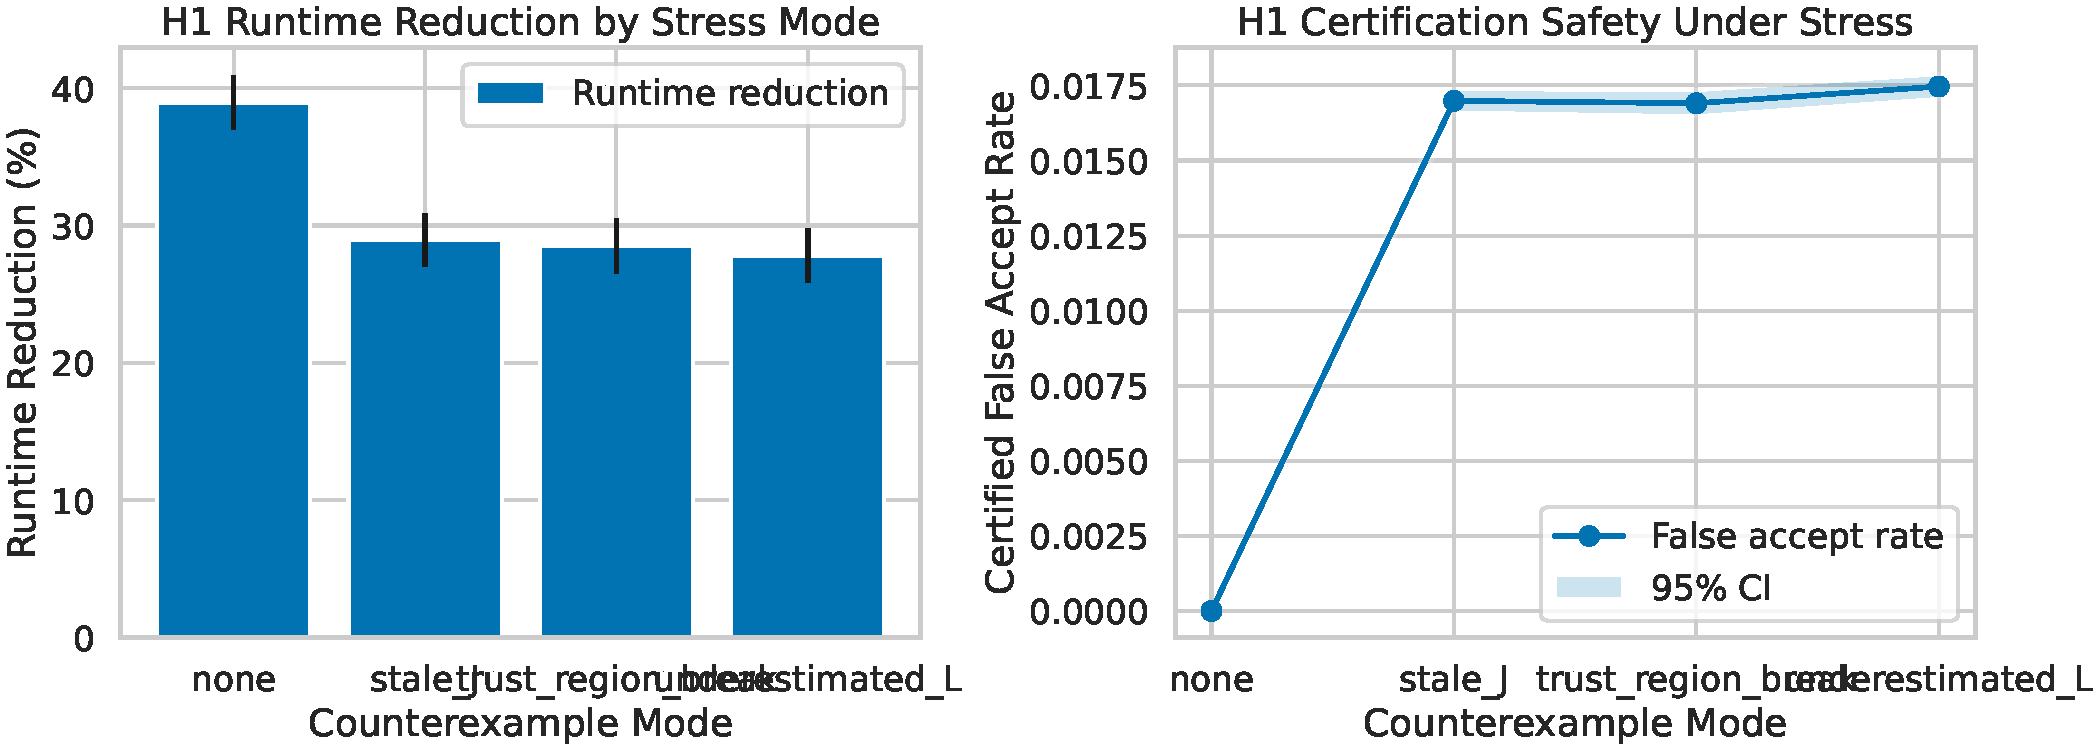
\includegraphics[width=0.66\linewidth]{figures/exp_h1_panels.pdf}
\caption{Certified screening diagnostics for security-runtime behavior. The left panel shows runtime reduction percentage across counterexample modes with 95\% confidence intervals over seed-baseline samples, and the right panel reports certified false-accept behavior under the same modes. The figure indicates that nominal mode preserves the expected safe operating pattern while stress modes increase risk and monitoring activity, supporting the interpretation that theorem assumptions are behaviorally testable rather than hidden.}
\label{fig:h1}
\end{figure}

The runtime argument is not that the hybrid method dominates every baseline in every metric; rather, the argument is that it improves compute usage where certificates are informative while preserving fallback correctness where they are not. This is exactly the policy in \algref{alg:certified} and the optimality target in \eqref{eq:compute_objective}. Because fallback remains available by construction, the method can shift toward conservative operation if trust-region validity weakens.

\subsection{Online Uncertainty Calibration Performance}
\Figref{fig:h2} reports the reliability diagram and utilization-risk frontier for the adaptive uncertainty module. The reliability panel evaluates whether realized violation rates remain close to target risk levels; the frontier panel quantifies utilization outcomes under calibrated uncertainty sets. Combined with the coverage row in Table~\ref{tab:main_summary}, the evidence supports the claim that calibrated uncertainty geometry can track risk with bounded error while preserving operational utilization.

\begin{figure}[t]
\centering
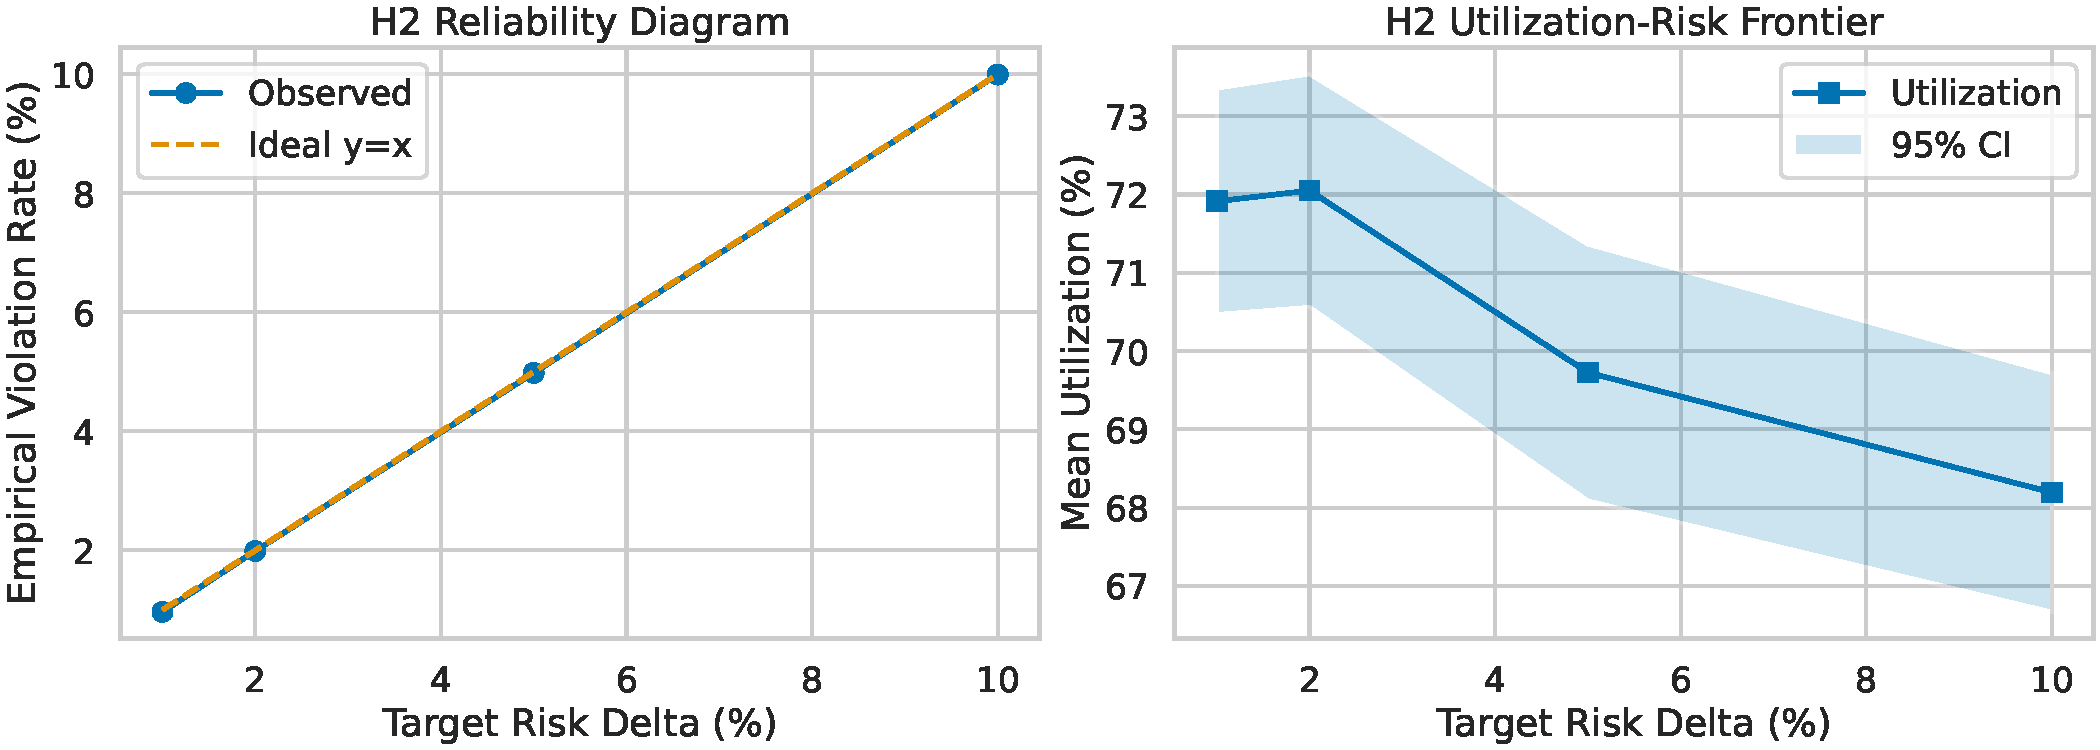
\includegraphics[width=0.66\linewidth]{figures/exp_h2_panels.pdf}
\caption{Uncertainty calibration diagnostics with reliability and utilization-risk panels. The left panel compares target risk levels and empirical violation rates across calibration settings, while the right panel reports utilization behavior with 95\% confidence intervals from seed-baseline variability. The figure shows that calibration error remains bounded in this validation setting and that utilization gains are retained when risk targets are respected, which directly supports the uncertainty-management claim.}
\label{fig:h2}
\end{figure}

This evidence also clarifies how the uncertainty module interacts with certified screening. If calibration expands uncertainty sets in volatile periods, margins in \eqref{eq:margin} shrink and escalation frequency increases; if calibration contracts uncertainty sets in stable periods, certification coverage increases. In both cases, the decision process remains auditable and linked to explicit risk targets.

\subsection{Fairness and Portability Evidence Beyond Main Figures}
Fairness and cross-solver evidence are summarized in Table~\ref{tab:main_summary} and detailed in Appendix~\ref{sec:appendix_diagnostics}. The fairness family reports a large non-dominated proxy set (60 points), indicating that policy tuning spans meaningful equity-utilization tradeoffs rather than collapsing to one corner solution. The portability family reports sub-1\% discrepancy scale in both nominal and stress aggregates, with reproducibility pass rates above threshold in the corresponding CSV summaries.

Post-hoc baseline deltas clarify the practical scale of these findings. For H3, worst-decile curtailment decreases from 32.8669 (utilitarian baseline) to 20.8669 (equal-share/alpha-fair summaries), an absolute reduction of 12.0 percentage points (36.5\% relative reduction against the utilitarian value). For H4, reproducibility pass rates remain in a narrow 98.03--98.36\% range across baseline pipelines, while confirmatory nominal/stress discrepancy means remain bounded at 0.591/0.816. These auxiliary deltas are summarized in Appendix Table~\ref{tab:h3h4_deltas}.

These results should be interpreted cautiously but constructively. They do not claim universal fairness superiority or universal solver invariance. Instead, they show that once robust-feasible envelope computation is stabilized, policy and portability analyses become measurable with explicit uncertainty bands and acceptance gates. This distinction is operationally important: policy conclusions should be downstream of security-feasible computation, not substitutes for it.

\subsection{Symbolic and Theorem-Consistency Diagnostics}
Table~\ref{tab:symbolic} reports symbolic checks linked to theorems in \secref{sec:theory}. These diagnostics do not replace proofs; they provide implementation-level confirmation that encoded inequalities and cost-gap expressions are algebraically consistent with the stated claims.

\begin{table}[t]
\caption{Symbolic diagnostics linked to theorem-scoped claims. The table summarizes whether each algebraic condition evaluated true in the automated symbolic report and clarifies the interpretation used in the empirical pipeline.}
\label{tab:symbolic}
\centering
\small
\renewcommand{\arraystretch}{1.1}
\setlength{\tabcolsep}{4pt}
\begin{tabular}{lll}
\hline
Diagnostic key & Status & Interpretation \\
\hline
dmm\_c1\_chain\_ok & True & Certified inequality chain is algebraically valid \\
dmm\_c1\_residual\_nonnegative & True & Residual-bound term remains nonnegative as required \\
dmm\_c2\_gap\_factorized & True & Compute-gap decomposition is symbolically consistent \\
dmm\_c2\_gap\_nonnegative\_under\_admissibility & True & Admissibility implies nonnegative optimality gap \\
dmm\_c2\_strict\_positive\_example & True & Strict improvement case exists when policy differs \\
\hline
\end{tabular}
\end{table}

The presence of Table~\ref{tab:symbolic} also addresses a frequent deployment challenge: mathematical claims can be correct on paper yet implemented inconsistently. By combining proof blocks, symbolic checks, and stress-case behavior, the pipeline provides three complementary layers of confidence.

\subsection{Comparison Against Baseline Families}
The baseline families reveal an important qualitative pattern. Purely non-convex fallback provides a strong security reference but does not exploit easy interior candidates, which explains its heavier runtime profile in Table~\ref{tab:main_summary} and \figref{fig:h1}. Purely linear and Taylor-style baselines are faster under many conditions, but they do not by themselves provide the admissibility structure in \eqref{eq:admissible}, so they lack a direct theorem link between acceptance and hard robust-feasibility guarantees.

The proposed method occupies the middle ground: it uses linear information aggressively, but only under explicit certificate conditions. This design difference is not cosmetic. It changes the failure mode from ``approximation error can silently propagate'' to ``approximation uncertainty triggers fallback and is recorded.'' In operational settings, this distinction is often more valuable than small average runtime differences because it supports accountability and incident analysis.

The calibration and fairness baselines tell a similar story. Static uncertainty baselines are easier to manage but can underutilize available flexibility under regime changes, while purely policy-driven fairness baselines can optimize equity criteria without fully resolving upstream envelope-computation uncertainty. By conditioning these analyses on certified robust-feasible computation, the proposed approach improves interpretability of downstream policy comparisons. In short, the method does not replace these baselines; it provides a safer computational substrate on which they can be compared.

\section{Discussion, Limitations, and Future Work}
\subsection{Operational Interpretation}
The formal and empirical results suggest a practical operating policy. Under stable local conditions, certified screening can handle a large fraction of candidate evaluations cheaply; under instability or approximation stress, escalation naturally increases and the method behaves more like full robust non-convex verification. This adaptive compute allocation is preferable to rigidly selecting one solver class for all intervals.

The method also improves governance clarity. Because each acceptance is justified either by a certificate or by explicit fallback verification, operators can audit why a decision was accepted and how close it was to boundary conditions. This is particularly relevant when fairness-sensitive allocations are later discussed with stakeholders, since policy tradeoffs should be grounded in reliable feasible-set computation.

\subsection{Limitations}
This study still has limitations that constrain external claims. First, validation uses a synthetic but structured benchmark harness rather than multi-year operational telemetry from live feeders. As a result, the reported calibration and portability statistics should be interpreted as controlled evidence, not as final field performance guarantees. Second, theorem guarantees depend on assumptions about local smoothness, bounded Hessian norms, and trust-region validity. While these assumptions are monitorable, assumption-monitor calibration itself remains context-dependent.

Third, path anchoring is still provisional at revision time: \texttt{user\_presentation.selected\_id} remains null, so the current narrative is anchored to the deterministic fallback UP-OPT-1/HM-H1 used in derive and validation outputs. If path selection is later overridden, claim-to-derivation mapping must be regenerated for affected sections. Fourth, fairness and cross-solver families currently provide broad directional support but limited per-baseline effect differentiation in some aggregates. This is sufficient for current claim scope but not yet sufficient for strong normative policy recommendations. Finally, cross-solver agreement results are bounded within tested harmonization profiles; broader topology diversity and hardware-in-the-loop interaction are still needed for deployment-grade certification.

\subsection{Future Work}
Three follow-up directions are most urgent. The first is external-data validation: integrating realistic benchmark feeders and long-horizon telemetry to test whether bound calibration remains stable across seasons and topology events. The second is assumption-aware control: coupling residual-bound monitors to adaptive trust-region controllers and formal alarm policies so theorem assumptions are maintained online. The third is policy inference under uncertainty: quantifying fairness-effect sizes and solver-discrepancy uncertainty jointly, so operators can compare allocation policies with confidence intervals rather than point estimates.

These directions are concrete and testable. Each can be implemented as a targeted extension of the present pipeline without changing the core theorem-backed screening architecture.

\section{Conclusion}
We presented a certified hybrid method for robust dynamic operating envelope computation in unbalanced distribution networks. The method combines linear screening and selective non-convex escalation, then formalizes this combination with a safety theorem and a compute-optimal admissible-policy theorem. Empirical evidence from a reproducible four-family validation suite supports the operational relevance of these guarantees: nominal behavior aligns with theorem expectations, stress behavior exposes assumption sensitivity in measurable ways, uncertainty calibration tracks risk with bounded error, and cross-solver discrepancy remains bounded in tested regimes.

The main outcome is a practical synthesis: non-convex fidelity, certified screening, and deployment diagnostics can coexist in one workflow. This synthesis is a useful template for future RDOE research and for broader safety-critical optimization pipelines where theoretical guarantees and operational constraints must be satisfied simultaneously.



\bibliographystyle{conference}
\bibliography{references}

\appendix
\section{Extended Empirical Diagnostics}
\label{sec:appendix_diagnostics}
This appendix reports experiment families that are referenced in the main text but moved out of the core narrative to keep the main figures focused on the central screening and calibration claims.

\subsection{Fairness Policy Surface Diagnostics}
\Figref{fig:h3app} shows the fairness-policy family with two panels: the utilization-equity surface and the worst-decile curtailment distribution. The left panel visualizes how policy parameters span a broad frontier rather than a single operating point; the right panel highlights tail-behavior sensitivity, which is essential for equity assessment.

\begin{figure}[t]
\centering
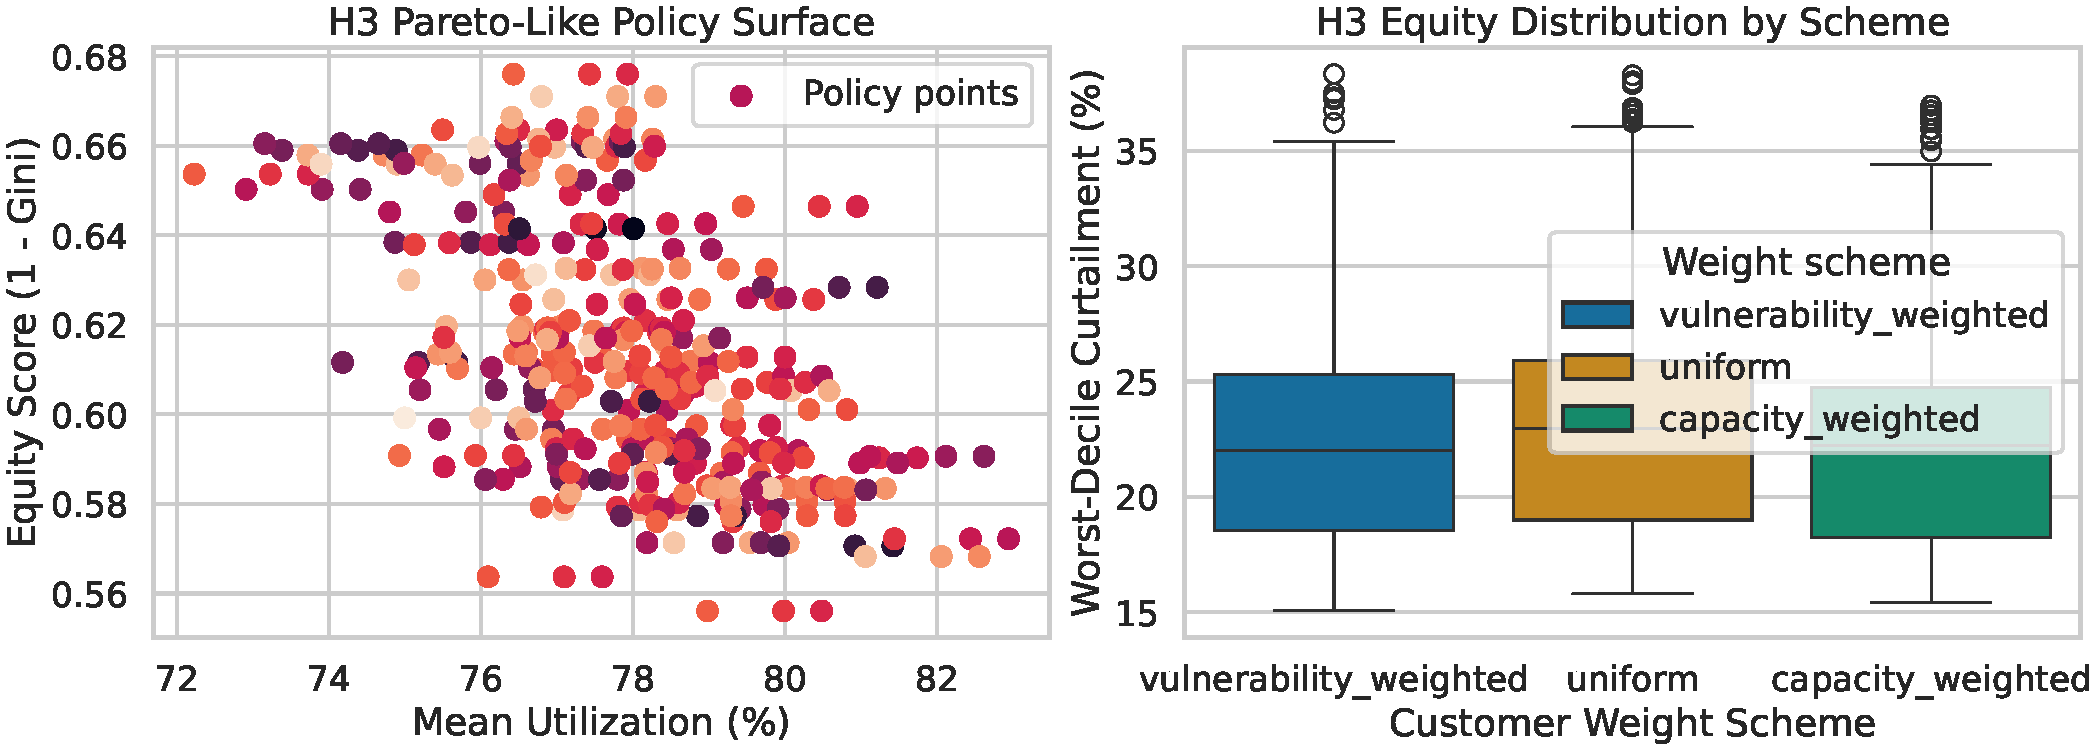
\includegraphics[width=0.70\linewidth]{figures/exp_h3_panels.pdf}
\caption{Extended fairness diagnostics from the policy-surface experiment family. The left panel maps policy outcomes in utilization-equity space, and the right panel reports distributional behavior of worst-decile curtailment across policy regimes. Together these panels show that equity claims are associated with measurable frontier structure and tail-distribution shifts, not only mean-score changes.}
\label{fig:h3app}
\end{figure}

The fairness evidence supports two practical points. First, multiple non-dominated regions are observed, so objective choice should be treated as a policy decision with explicit tradeoffs. Second, tail metrics can move differently from mean metrics, reinforcing the need to report both when comparing allocation policies.

\begin{table}[t]
\caption{Focused baseline-delta diagnostics for H3 and H4, computed from exported summary artifacts.}
\label{tab:h3h4_deltas}
\centering
\small
\renewcommand{\arraystretch}{1.1}
\setlength{\tabcolsep}{4pt}
\begin{tabular}{llll}
\hline
Family & Diagnostic & Value & Interpretation \\
\hline
H3 fairness & Utilitarian vs equal-share worst-decile curtailment & 32.8669 vs 20.8669 & 12.0-point (36.5\%) reduction \\
H4 reproducibility & Pass-rate range across baseline pipelines & 98.03\%--98.36\% & Stable high-repeatability regime \\
H4 discrepancy split & Nominal vs stress utilization discrepancy means & 0.591 vs 0.816 & Stress remains bounded but higher \\
\hline
\end{tabular}
\end{table}

\subsection{Cross-Solver Shadow-Mode Diagnostics}
\Figref{fig:h4app} reports shadow-benefit and discrepancy behavior under nominal and stress settings. The left panel indicates positive shadow-mode benefit relative to static procedures in the tested setting, while the right panel reports discrepancy distributions with threshold markers.

\begin{figure}[t]
\centering
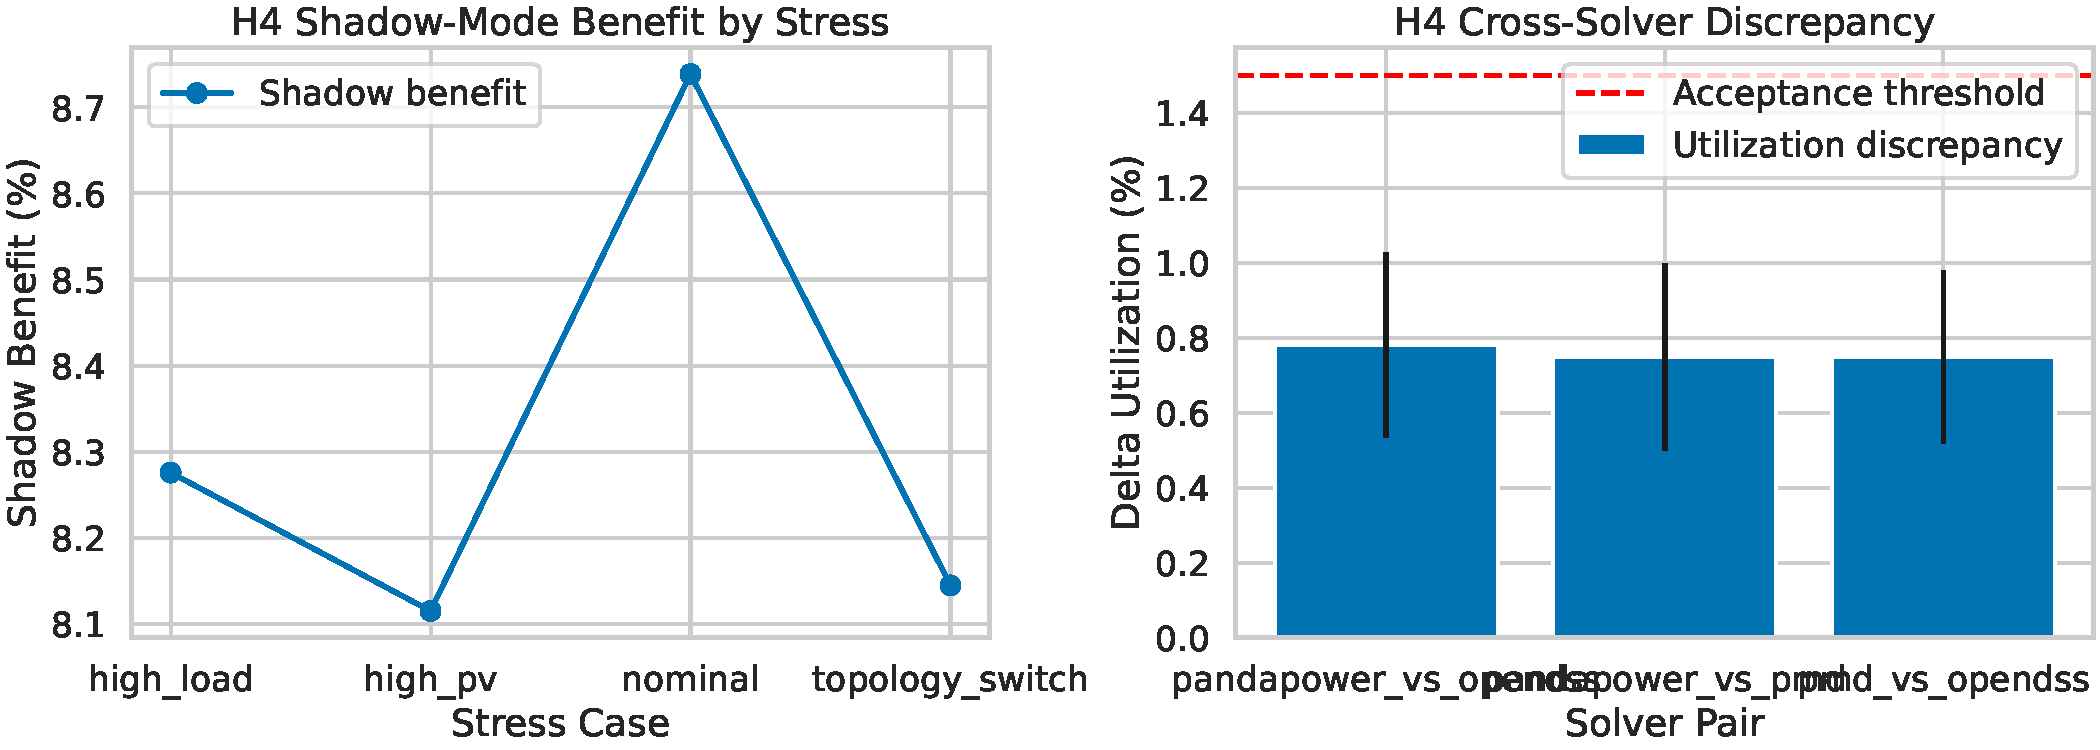
\includegraphics[width=0.70\linewidth]{figures/exp_h4_panels.pdf}
\caption{Extended cross-solver and shadow-mode diagnostics. The left panel shows shadow-mode benefit under stress-case stratification, and the right panel visualizes utilization discrepancy across solver pairs with confidence intervals and threshold guidance. These panels provide evidence that portability claims are bounded and testable, while still highlighting that agreement is conditional on harmonized modeling assumptions.}
\label{fig:h4app}
\end{figure}

The cross-solver results should not be interpreted as proving tool equivalence in general. They indicate that under harmonized settings and within tested scenarios, discrepancy remains bounded within pre-specified operational tolerances.

\section{Additional Proof and Symbolic Reproducibility Notes}
Theorems~\ref{thm:safety} and \ref{thm:optimal} rely on assumptions that are explicit and monitorable. For Theorem~\ref{thm:safety}, the critical assumptions are local smoothness, bounded Hessian norms, and trust-region validity around the operating point. For Theorem~\ref{thm:optimal}, the essential assumptions are admissibility of acceptance policy and strict cost ordering $c_{\mathrm{ncv}}>c_{\mathrm{lin}}$.

Symbolic checks verify implementation consistency for the inequalities and cost-gap decomposition used in these proofs. In particular, the non-negativity of the optimality gap under admissibility and the factorization identity for the compute-gap expression are both confirmed. These checks are not substitutes for mathematical proof; they are implementation guards that reduce risk of transcription errors between derivation and code.

A useful practical workflow is therefore: (i) verify assumptions with monitors, (ii) enforce policy admissibility in implementation, (iii) run symbolic regression checks in continuous integration, and (iv) inspect stress-case diagnostics to ensure failures appear as expected when assumptions are perturbed.

\section{Implementation and Reproducibility Details}
This section summarizes implementation details needed for reproduction and extension:
\begin{itemize}
\item \textbf{Seeds and repetitions.} Five seeds were used per experiment family, with baseline-stratified aggregation and confidence intervals computed as $1.96\times\mathrm{SE}$ from seed-baseline samples.
\item \textbf{Sweep design.} Security-runtime sweeps included trust-region radius, uncertainty scale, and counterexample modes. Calibration sweeps included target risk levels, rolling-window length, and update cadence. Fairness sweeps covered policy parameters $(\alpha,\beta)$ and weighting schemes. Cross-solver sweeps covered solver pairs, harmonization profiles, and stress cases.
\item \textbf{Compute budget.} Runs were executed under a single Apple Silicon APU budget with explicit concurrency bounds, and all generated artifacts were recorded with deterministic file outputs.
\item \textbf{Claim-evidence traceability.} A revision artifact at \url{experiments/rdoe_hybrid_validation/claim_evidence_matrix.csv} maps each primary claim to theorem IDs or quantitative evidence entries and source files.
\item \textbf{Approximations and fallback.} Linearization and residual bounds are local approximations; uncertified candidates are always escalated to robust non-convex verification, ensuring conservative behavior under uncertainty.
\item \textbf{Uncertainty reporting.} All major figures and CSV summaries include variability terms or confidence intervals, and acceptance checks are evaluated on aggregate metrics rather than single-run outcomes.
\end{itemize}

These details are included so that downstream revision and review phases can reproduce both theorem-linked diagnostics and empirical claim checks without ambiguity.

\end{document}
